% -----------------------------------------------------------------------------
% Implementation
% -----------------------------------------------------------------------------
\chapter{Implementation}
\label{chap:implementation}
\section{Image Source Method}
The implementation of the image source model will unfold in several steps. Building up from a rudimentary to a more complex and realistic implementation.
\subsection{Images Source Method with 4 walls - image order 1}
We start by modeling a simple room with only 4 walls (no ceiling or floor) with a receiver positioned at the point (single source positioned at the point $P(1,1,1)$ and its reflection of the first order relative to the walls as seen in figure \ref{fig:ism_4_1_geo}\\
\begin{figure}
    \centerline{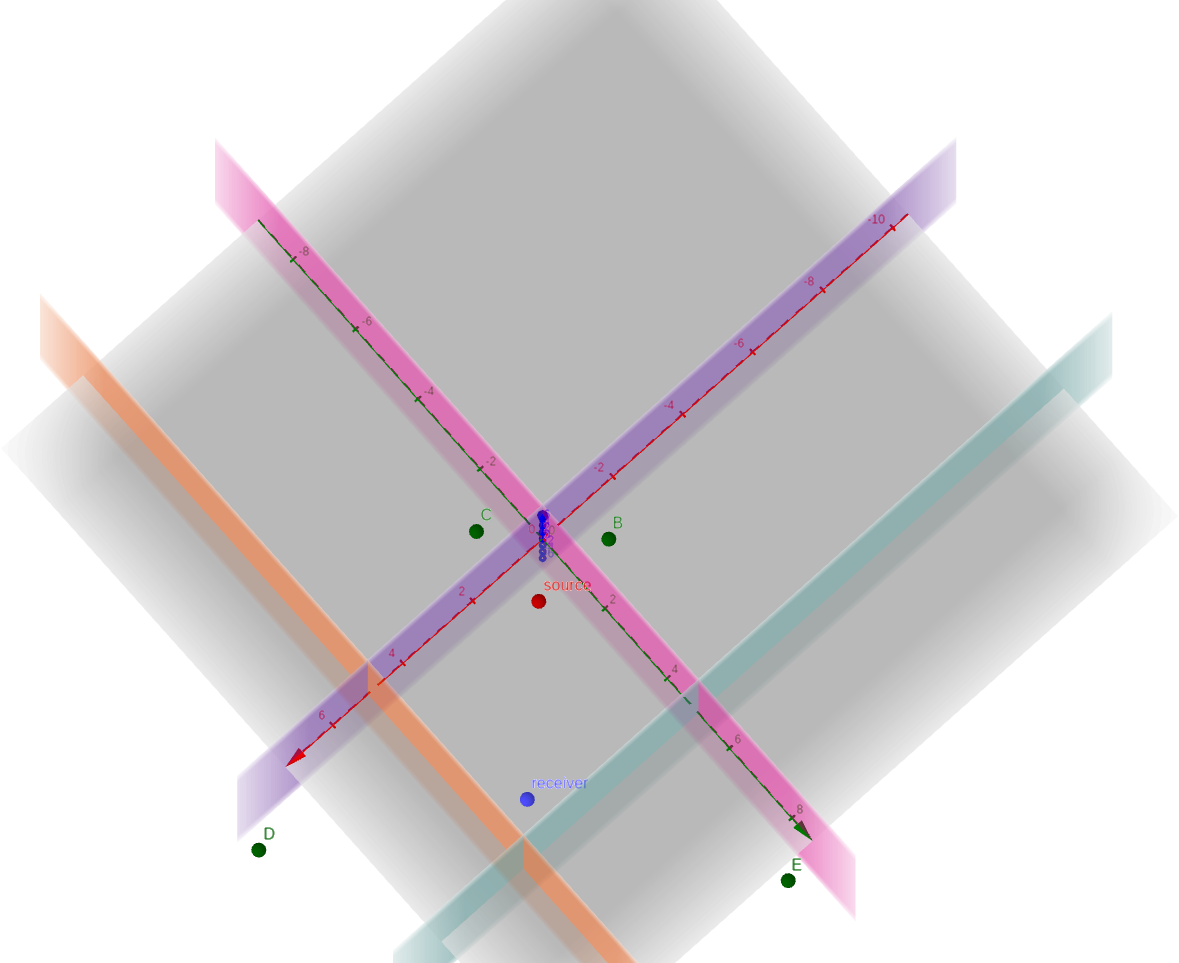
\includegraphics[width=1.3\textwidth,keepaspectratio]{LaTeX/images/geometrie/ism_4_walls_order_1.png}}
    \caption{Source and receiver in room with 4 walls and reflections of order 1}
    \label{fig:ism_4_1_geo}
\end{figure}
When adding the pressure waves emitted by the source and all the source images we get the pressure deviation perceived at the receiver as seen in figure \ref{fig:ism_4_1_mat}
\begin{figure}

    \centerline{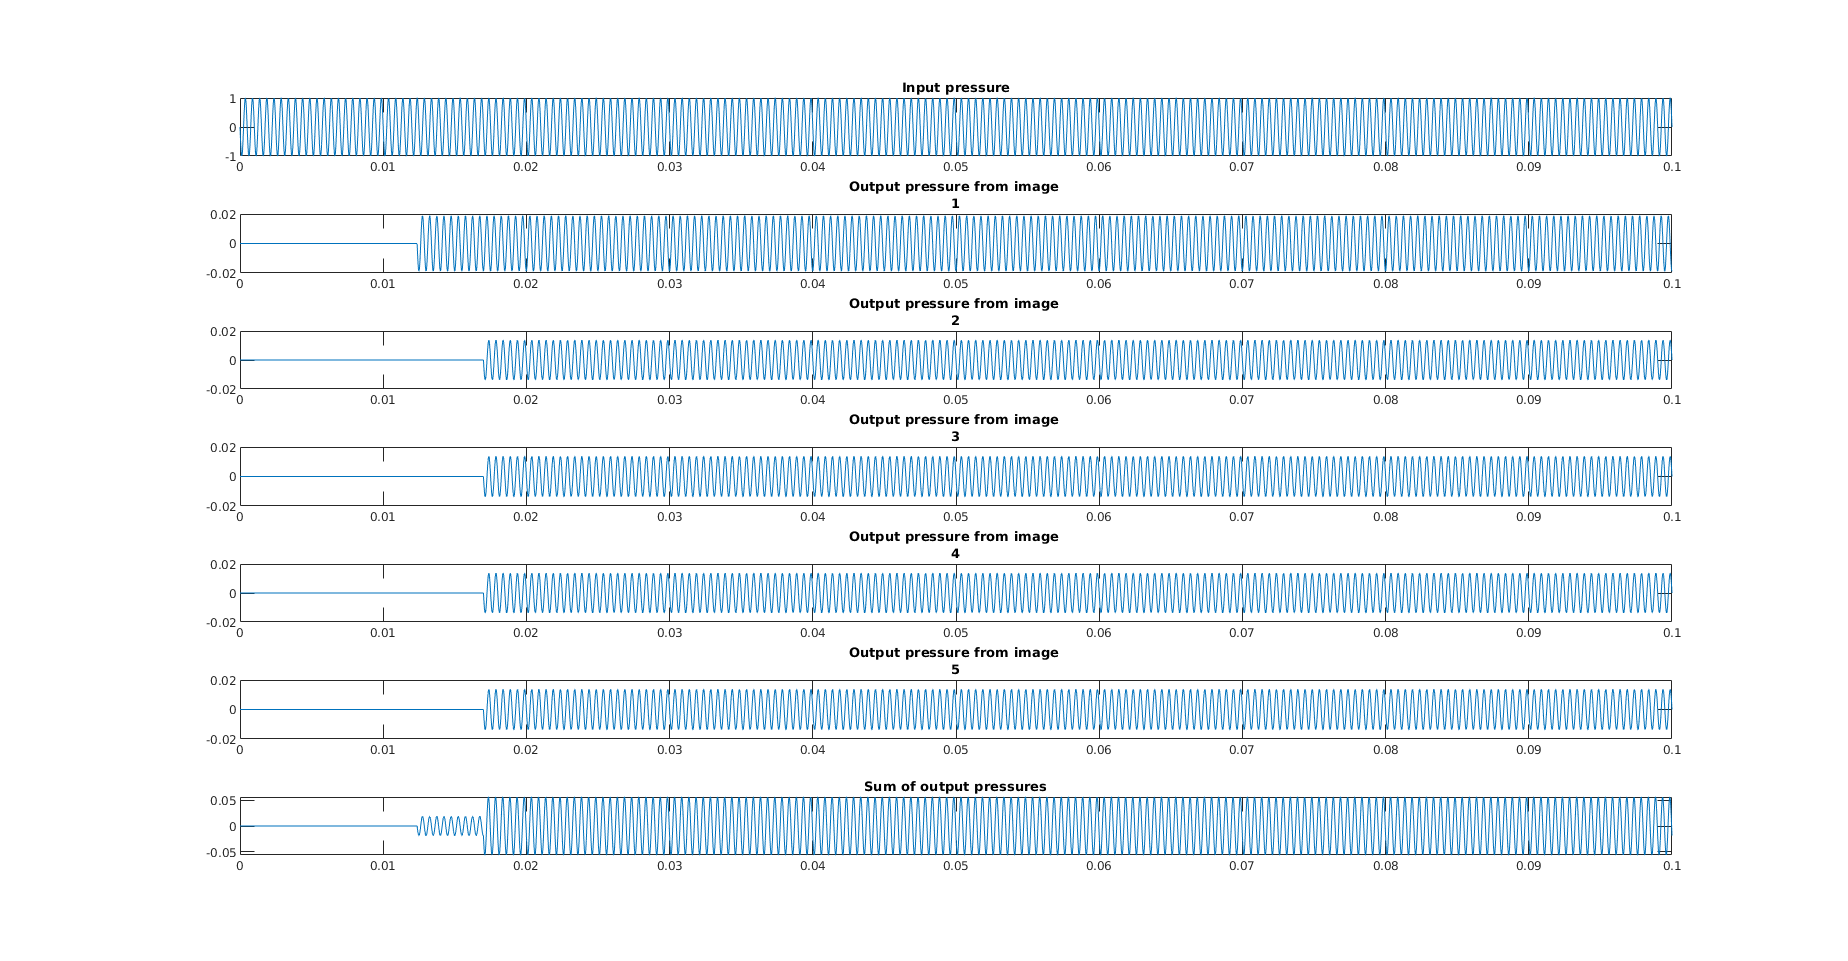
\includegraphics[width=1.8\textwidth,keepaspectratio]{LaTeX/images/plots/matlab_4_walls_order_1.png}}
    \caption{Pressure deviation perceived at receiver emitted by source and source images}
    \label{fig:ism_4_1_mat}
\end{figure}
\subsection{Image Source Method with 4 walls - image order 2}
In the next step the same scenario is computed for an image order 2. Each image is produces itself one image relative to each wall as seen in figure \ref{fig:ism_4_2_geo}\\
\begin{figure}
    \centerline{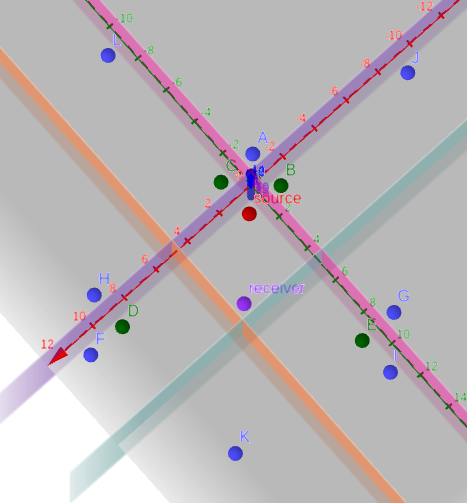
\includegraphics[width=1\textwidth,keepaspectratio]{LaTeX/images/geometrie/ism_4_walls_order_2.png}}
    \caption{Source and receiver in room with 4 walls and reflections of order 1}
    \label{fig:ism_4_2_geo}
\end{figure}
The resulting pressure wave deviation can be seen in figure \ref{fig:ism_4_2_mat}
\begin{figure}

    \centerline{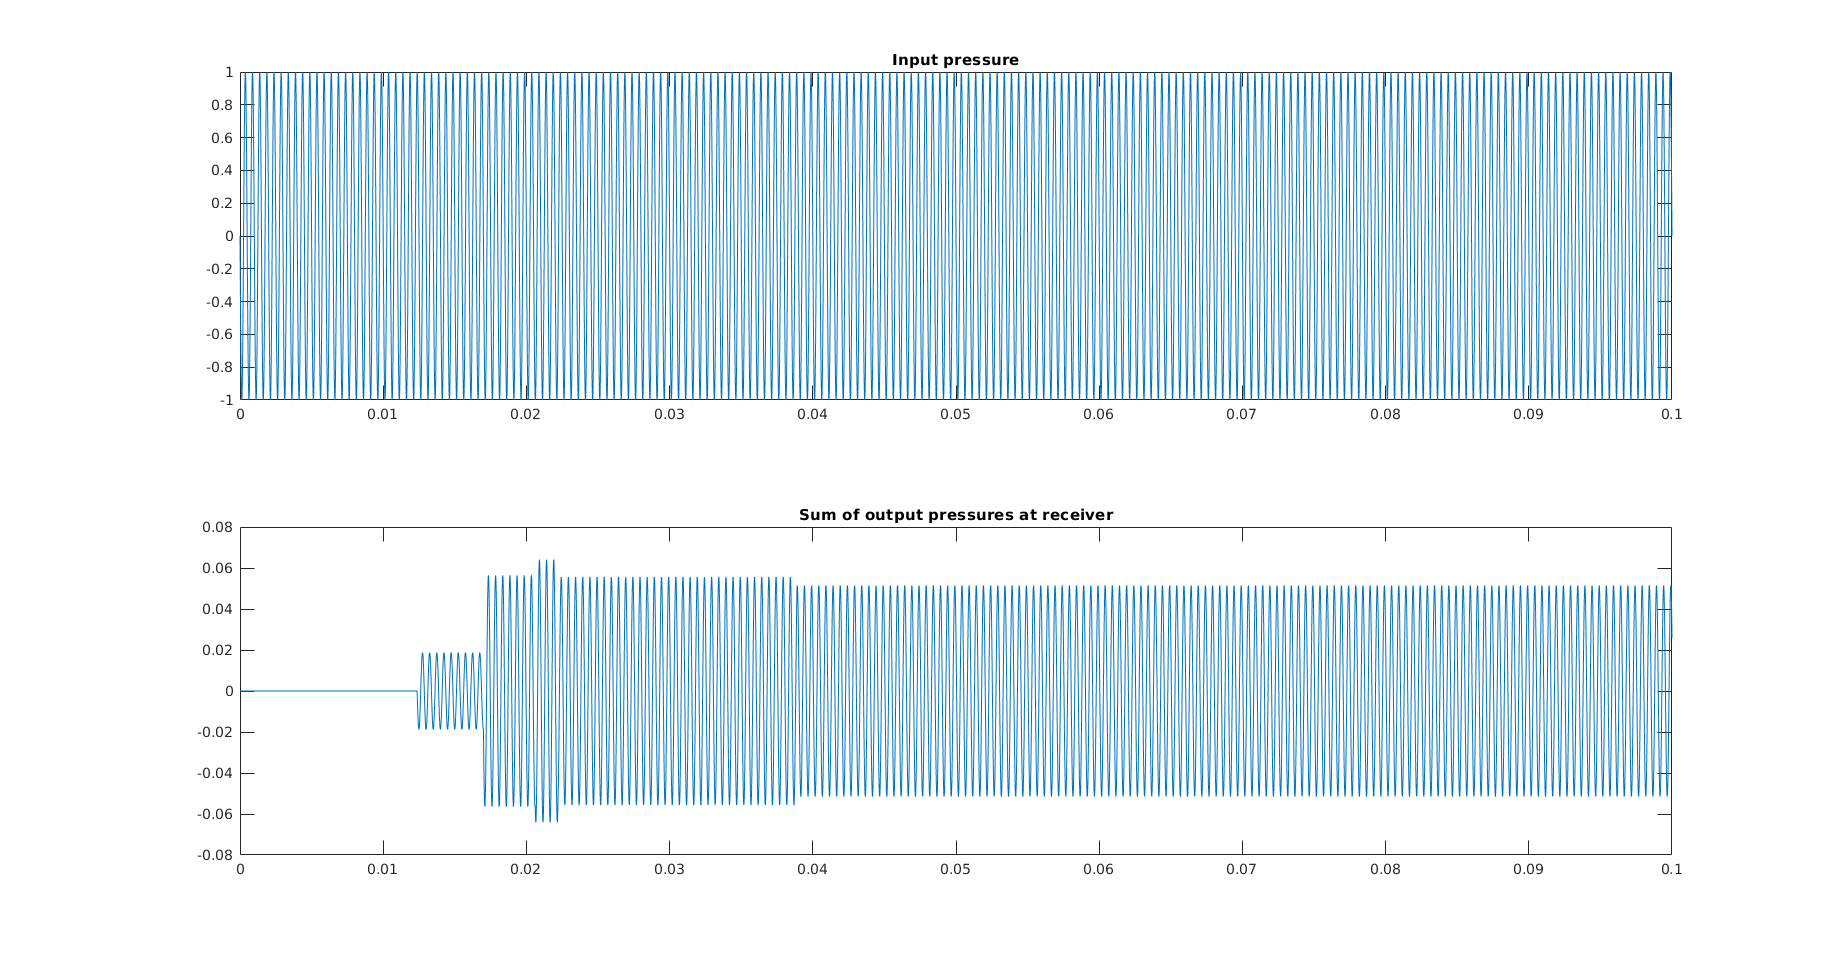
\includegraphics[width=1.5\textwidth,keepaspectratio]{LaTeX/images/plots/matlab_4_walls_order_2.png}}
    \caption{Pressure deviation perceived at receiver emitted by source and source images}
    \label{fig:ism_4_2_mat}
\end{figure}
\subsection{Image Source Method with 4 walls + ceiling + floor - image order 2}
Adding a ceiling and a floor we get even more images which leads to a very busy 3D-Model in figure \ref{fig:ism_4_2_2_geo}\\
\begin{figure}
    \centerline{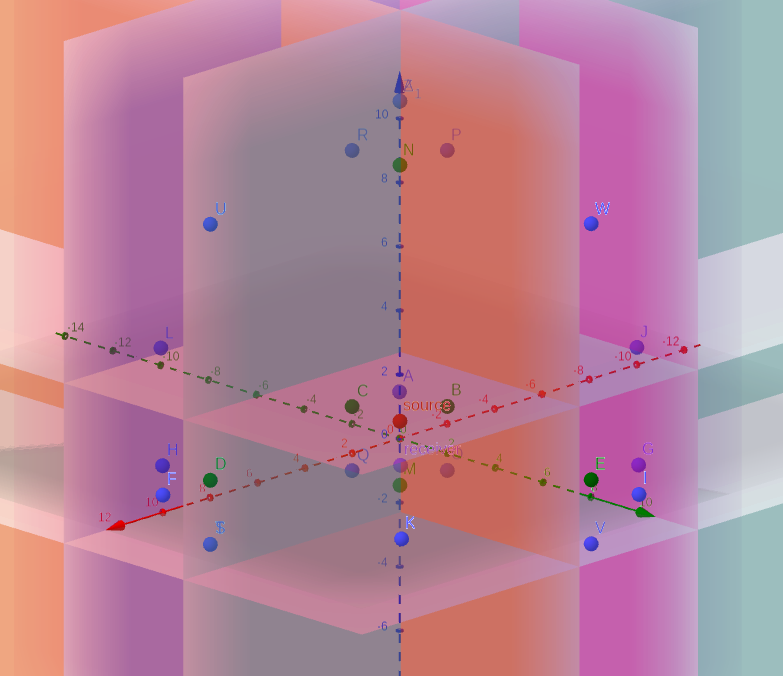
\includegraphics[width=1\textwidth,keepaspectratio]{LaTeX/images/geometrie/ism_4_walls_2_order_2.png}}
    \caption{Source and receiver in room with 4 walls + ceiling + floor and reflections of order 1}
    \label{fig:ism_4_2_2_geo}
\end{figure}
And the pressure deviation at receiver as seen in figure \ref{fig:ism_4_2_2_mat}
\begin{figure}

    \centerline{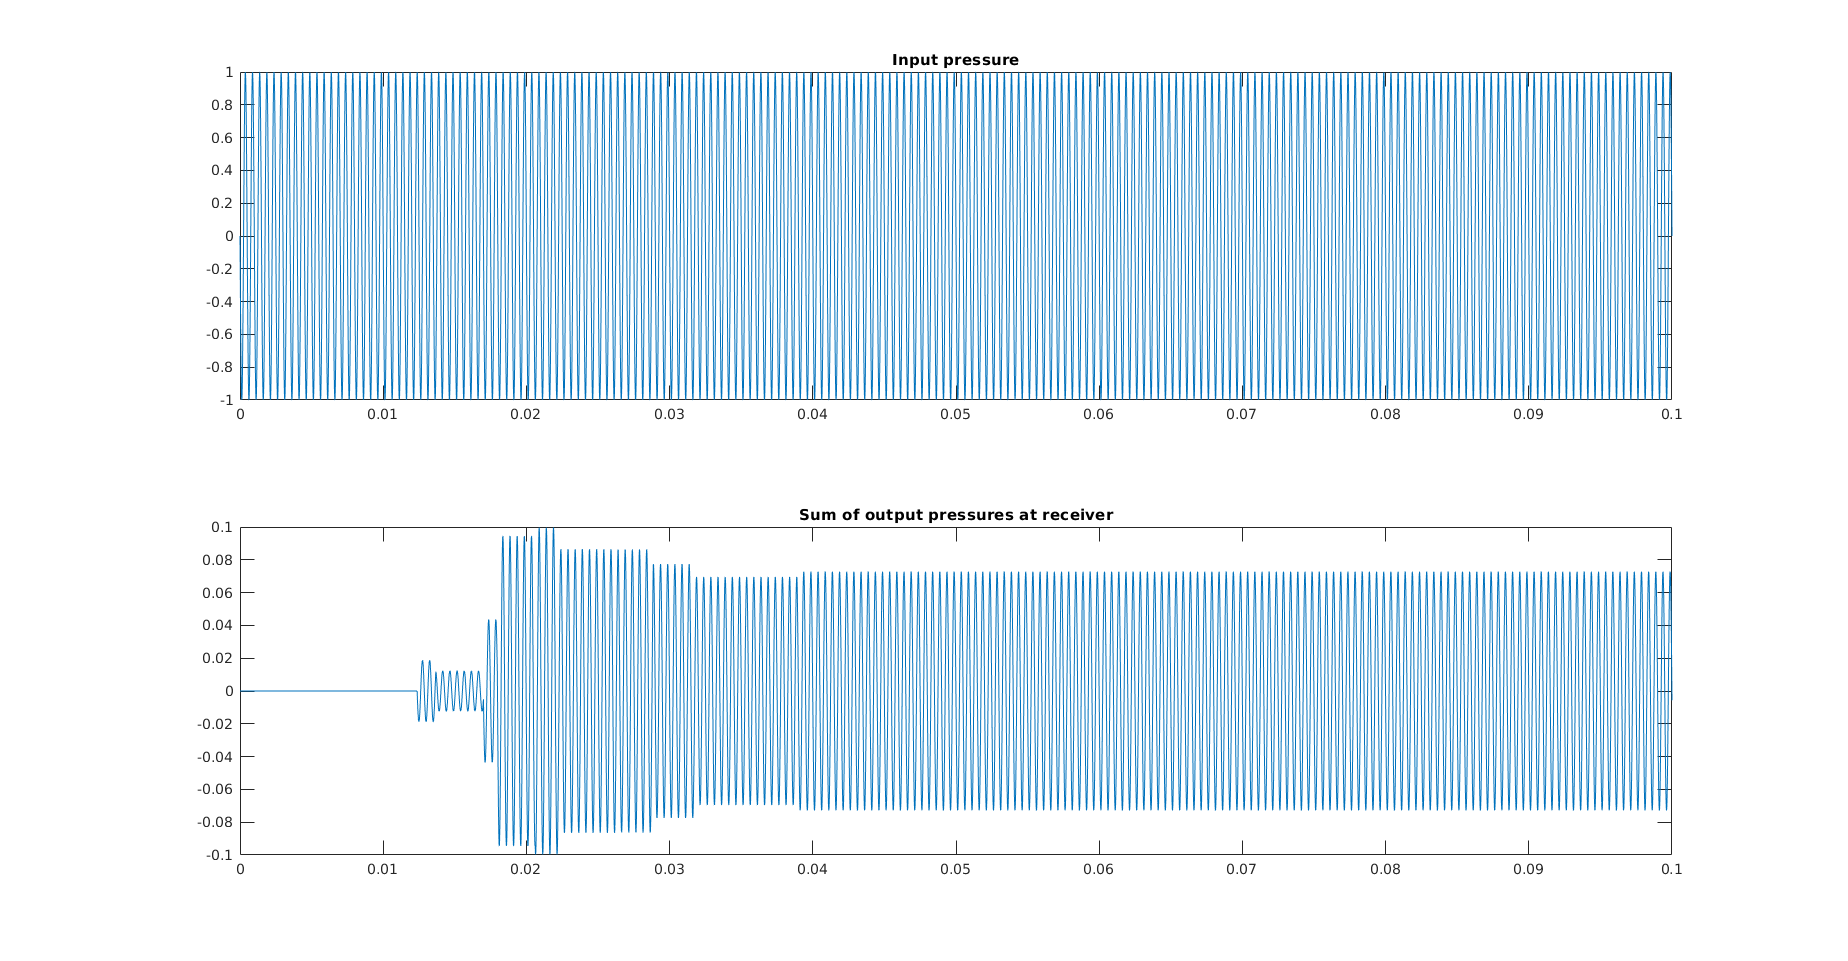
\includegraphics[width=1.5\textwidth,keepaspectratio]{LaTeX/images/plots/matlab_4_walls_2_order_2.png}}
    \caption{Pressure deviation perceived at receiver emitted by source and source images}
    \label{fig:ism_4_2_2_mat}
\end{figure}